\documentclass[11pt]{article} % For LaTeX2e
\usepackage{rldmsubmit,palatino}
\usepackage{graphicx}

\title{Modular Inverse Reinforcement Learning on Human Motion}

\author{
Shun Zhang\\
Department of Computer Science\\
University of Texas at Austin\\
Austin, TX 78712 \\
\texttt{menie482@cs.utexas.edu} \\
\And
Matthew Tong \\
Center for Perceptual Systems\\
University of Texas at Austin\\
Austin, TX 78712 \\
\texttt{mhtong@gmail.com} \\
\AND
Mary Hayhoe \\
Center for Perceptual Systems\\
University of Texas at Austin\\
Austin, TX 78712 \\
\texttt{hayhoe@utexas.edu} \\
\And
Dana Ballard \\
Department of Computer Science\\
University of Texas at Austin\\
Austin, TX 78712 \\
\texttt{dana@cs.utexas.edu} \\
\\
}

% The \author macro works with any number of authors. There are two commands
% used to separate the names and addresses of multiple authors: \And and \AND.
%
% Using \And between authors leaves it to \LaTeX{} to determine where to break
% the lines. Using \AND forces a linebreak at that point. So, if \LaTeX{}
% puts 3 of 4 authors names on the first line, and the last on the second
% line, try using \AND instead of \And before the third author name.

\newcommand{\fix}{\marginpar{FIX}}
\newcommand{\new}{\marginpar{NEW}}

\begin{document}

\maketitle

\begin{abstract}
%The \emph{abstract} should be a maximum of 2000 characters of text, including
%spaces (no figure is allowed).
\end{abstract}

\keywords{
Reinforcement learning, human motion, inverse learning
}

\startmain % to start the main 1-4 pages of the submission.

\section{Introduction}

Human is able to learn accomplishing complicated tasks much faster than machines
can do. However, most of the tasks can be decomposed into subtasks. A human may
already have the capacity to accomplish the subtasks. He simply transfers the
knowledge of the subtasks and integrate them for the objective task. For example,
when a human learns to drive, he has much prior domain knowledge to help him
with this objective task. He integrates his skills of controlling the velocity,
avoiding other vehicles, navigating, responding to traffic lights, and so on.

Similar ideas are also adopted in the learning literature. Reinforcement learning
suffers from the curse of dimensionality. It is inefficient for a learning agent
to learn a complicated task from scratch. So learning algorithms including
hierarchical reinforcement learning \cite{dietterich2000hierarchical}, modular
reinforcement learning \cite{sprague2003multiple} are proposed. They also
decompose the objective task into subtasks. The learning algorithms first learn
the subtasks independently, then learn how to combine these subtasks.

A natural question to ask is how human integrates skills for subtasks, and
whether we can use the same method for integrating subtasks in reinforcement
learning problems. In this paper, we analyze human's behavior of
accomplishing a task composite of various subtasks. We collected human motion
data and try to interpret the behavior using a way of
inverse reinforcement learning. With the best of our knowledge, this approach is
novel in the literature.

This paper is organized as follows. Section~\ref{sec:domain} introduces the
domain of the composite task that we collected human data. Section~\ref{sec:rl}
describes the main algorithm, modular inverse reinforcement learning. We report
our experiment results in Section~\ref{sec:exp}, and conclude in
Section~\ref{sec:conclude}.

\section{Multi-objective Sidewalk Domain}
\label{sec:domain}

\begin{figure}[h!]
\centering
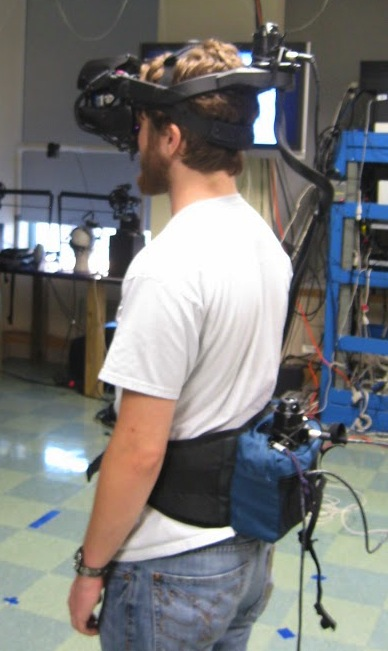
\includegraphics[height=6cm]{human.jpg}
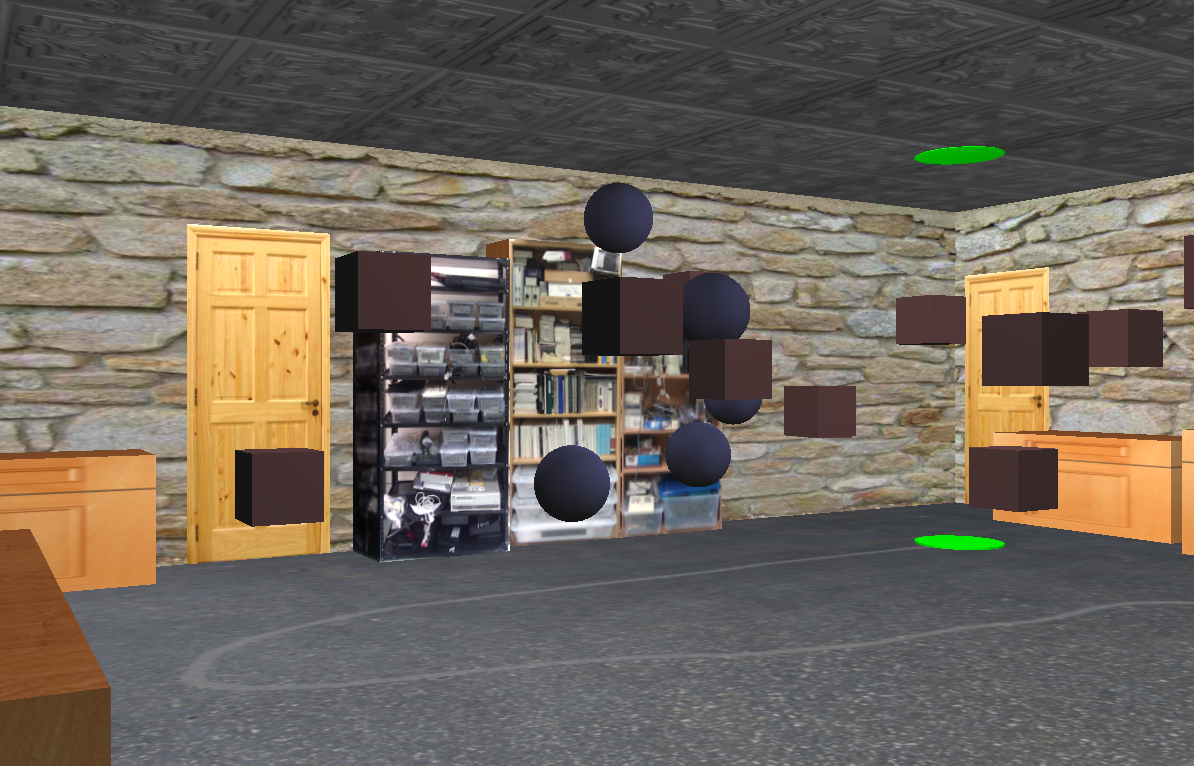
\includegraphics[height=6cm]{env.png}
\caption{(Left) A volunteer with head tracker, virtual reality displayer, and
body tracker.  (Right) The environment the human can see through the displayer.}
\label{fig:avatar}
\end{figure}

Figure~\ref{fig:avatar} shows the domain that we use in this paper. The red
cubes represent obstacles, that the player would be punished if running
into. The blue balls represent targets, that the player would be rewarded if
collected. There is also a gray path on the ground that the player can follow.
Naturally, this domain has three subtasks, 1) following the path, 2)
collecting targets, 3) avoiding obstacles.
This is an experiment used in the
literature to evaluate modular reinforcement learning
\cite{rothkopf2013modular}.
We ask our volunteers to have trackers and virtual reality displayers equipped. He
can see the envrionment through the displayer in front of his eyes. So he can
walk as if he is walking in the virtual domain.

We will evaluate four different tasks. {\bf Task 1}, following the path only, and
ignoring other objects. {\bf Task 2}, following the path, while avoid the obstacles.
{\bf Task 3}, following the path, while attain targets when possible. {\bf Task 4},
following the path, collecting the targets and avoiding obstacles
simultaneously.
We conducted experiments to ask volunteers to accomplish different tasks and
recorded their trajectories. The human data are collected by the Center for
Perceptual Systems at University of Texas at Austin.

If the player observes the distance and angle to an object, he is expected to
know the optimal action to avoid or pursue it. This decision is also Markov.
Therefore, the question would be, if we have trained modules for these three
subtasks, could they be integrated to match human's behavior?

\section{Modular Inverse Reinforcement Learning}
\label{sec:rl}

We need some basic concepts in reinforcement learning to proceed. For a state, action
pair, $s$ and $a$, $Q(s, a)$ evaluates the utility of taking action $a$ from
state $s$. The {\em policy} of a state is the action with the maximum Q
value \cite{rl}. So how to we determine the global policy from the modules, or
subtasks? In the literature, work has been done to integrate the Q function
\cite{koller1999computing} or compromise on policies directly
\cite{thomas2012motor}.

Here, we assume that the global Q function is a weighted sum of all $Q_i$, where
$Q_i$ is the Q function for i-th module.
$$Q(s, a) = \sum_i w_i Q_i (s_i, a)$$
where $w_i$ is the weight of the i-th sub-MDP. $w_i \geq 0, \sum_i w_i = 1$.
$s_i$ denotes the decomposition of $s$ in the i-th module.

Different weights can yield different performance. Let $w_1, w_2, w_3$ be
weights for the task of target collection, obstacle avoidance, and path
following, respectively. Let $w$ be the vector of $(w_1, w_2, w_3)$. An agent
with $w = (1, 0, 0)$ only collects targets, and one with $w = (0, 0.5, 0.5)$ may
avoid the obstacles and follow the path.

To obtain the weights given the samples, we need to use the Inverse Modular
Reinforcement Learning technique \cite{rothkopf2013modular}. We use a maximum
likelihood method here.
\begin{equation}
\label{eq:irl}
\max_w \prod_t \frac{e^{\eta Q(s^{(t)}, a^{(t)})}}{\sum_b e^{\eta Q(s^{(t)}, b)}}
\end{equation}
where $s^{(t)}$ is the state at time $t$, and $a^{(t)}$ is the action at time
$t$, which are both from samples. $Q(s, a) = \sum_i w_i Q_i(s_i, a)$, as defined
before. $\eta$ is a hyperparameter that determines the consistency of human's
behavior. The larger $\eta$ is, the algorithm is more likely to overfit the data.

The intuition of Equation~\ref{eq:irl} is that if an action is observed from the
sample, then the Q value of taking that action should be larger compared to Q
values of taking other actions.

\section{Experiments}
\label{sec:exp}

We train the modules first to get $Q_i$ before running the inverse reinforcement
learning algorithm. For each module, the agent only considers the closest target
and the closest obstacle. For the path module, the path is defined as segments
of waypoints, so the closest waypoint is considered. The agent takes the
distance and angle to the closest objects as the state representation.

To make our weights represent the significance of the modules, we
normalize the sub-MDPs with the unit (positive or negative) rewards. The reward
is 1 for collecting a target, -1 for running into an obstacle. We define the
value function directly for the path module to have a path following
performance, as it is tricky to give reward for such performance.

We make some constraints on our learning agent to make it walk like a human.
We can find in the human trajectories that humans walk smoothly. They don't turn
sharply.  Our agent is only allowed to do three actions --- going straight ahead,
turning left with a small step, and turning right with a small step.

\begin{figure}[h!]
\centering
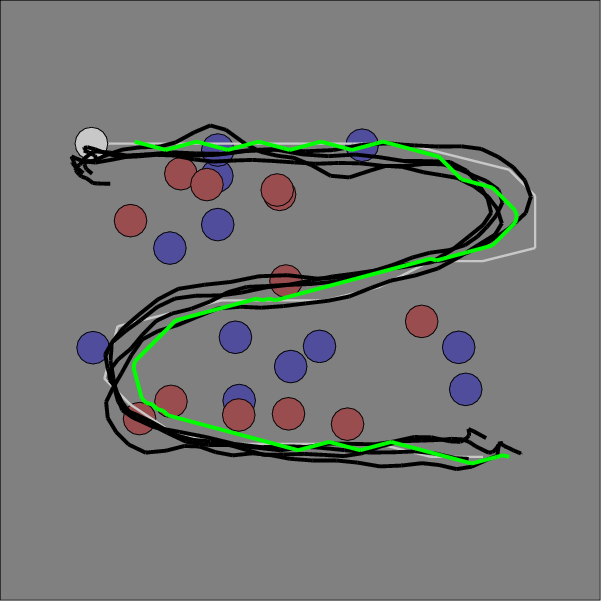
\includegraphics[width=0.24\textwidth]{task_1.png}
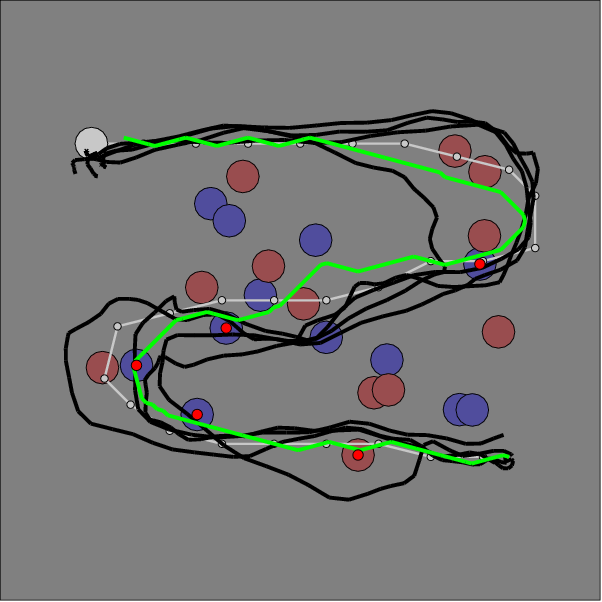
\includegraphics[width=0.24\textwidth]{task_2.png}
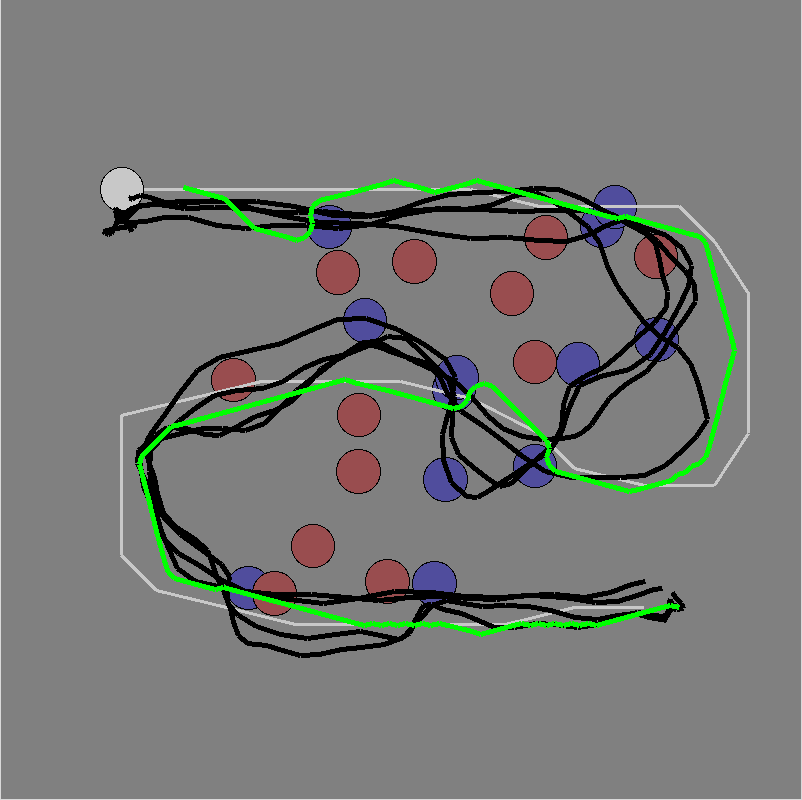
\includegraphics[width=0.24\textwidth]{task_3.png}
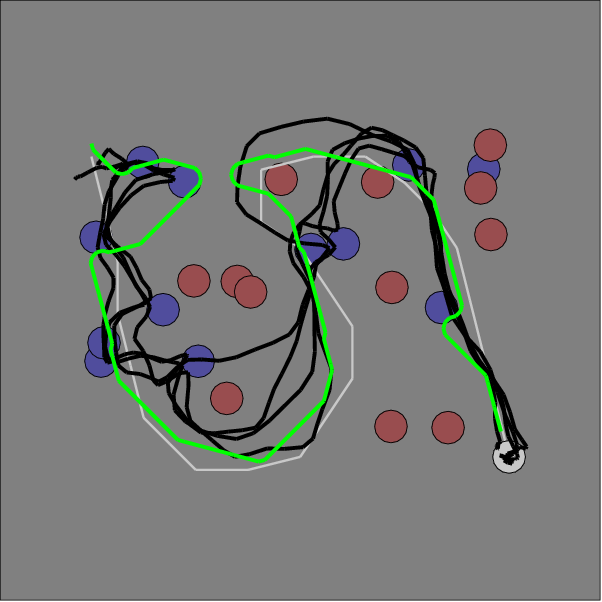
\includegraphics[width=0.24\textwidth]{task_4.png}
\caption{The trajectories of humans and our agent in four different tasks. From
left to right are Task 1 to Task 4. The active modules should be (Path),
(Obstacle + Path), (Target + Path), (Target + Obstacle + Path), respectively.}
\label{fig:exp}
\end{figure}

\begin{table}[h!]
\centering
\begin{tabular}{| l| l| l |}
\hline
Average by Task & Num Targs Hit & Num Obst Hit\\
\hline
1 & 2.34 &  2.13\\
\hline
2 & 3.03 &  \bf{0.13}\\
\hline
3 & \bf{10.19} & 2.28\\
\hline
4 & \bf{9.88} &  \bf{0.03}\\
\hline
\end{tabular}
\caption{Number of targets hit and number of obstacles hit of the humans.}
\label{tb:human}
\end{table}

\begin{table}[h!]
\centering
\begin{tabular}{| l| l| l |}
\hline
Average by Task & Num Targs Hit & Num Obst Hit\\
\hline
1 & 1.25 & 1.62\\
\hline
2 & 3.62 & \bf{2.37}\\
\hline
3 & \bf{5.14} & 3.14\\
\hline
4 & \bf{5.00} & \bf{2.00}\\
\hline
\end{tabular}
\caption{Number of targets hit and number of obstacles hit of the learning agent.}
\label{tb:agent}
\end{table}

We report the results in Figure~\ref{fig:exp}, same as Figure~\ref{fig:avatar},
the red circles are obstacles. The blue circles are targets. The gray lines are
the path. The black lines are trajectories of human --- each line represents one
human trajectory.
Using the weights derived from the algorithm, the trajectories of our agents are
drawn in green color.

Although humans don't agree each other on how to avoid obstacles or collecting
targets, our agent can figure out what the humans are doing, and perform a
similar trajectory. Table~\ref{tb:human} and Table~\ref{tb:agent} evaluate the
performance by showing the number of targets hit and number of obstacles hit.
Note that the numbers bold-ed are active modules in the corresponding task. We
can observe that humans still do better than our agent in these tasks.

\begin{figure}[h!]
\centering
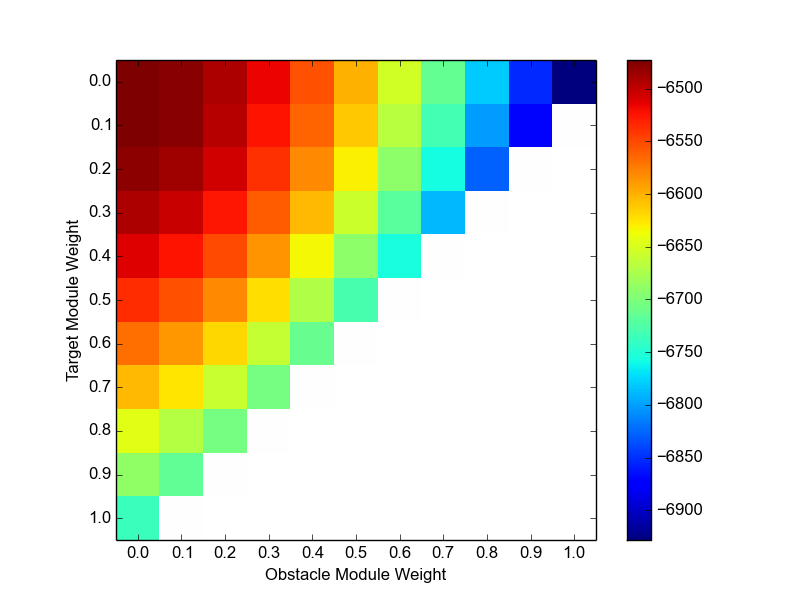
\includegraphics[width=0.4\textwidth]{objValuesTask1.png}
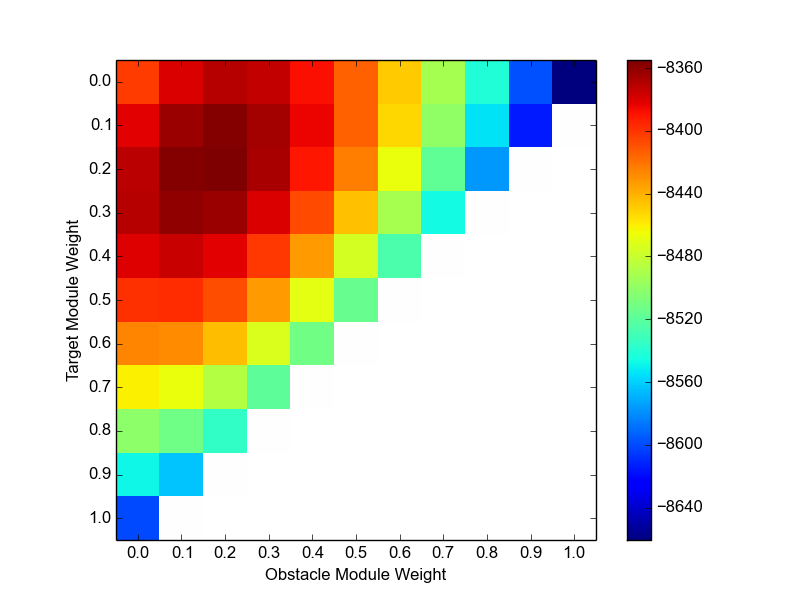
\includegraphics[width=0.4\textwidth]{objValuesTask2.png}
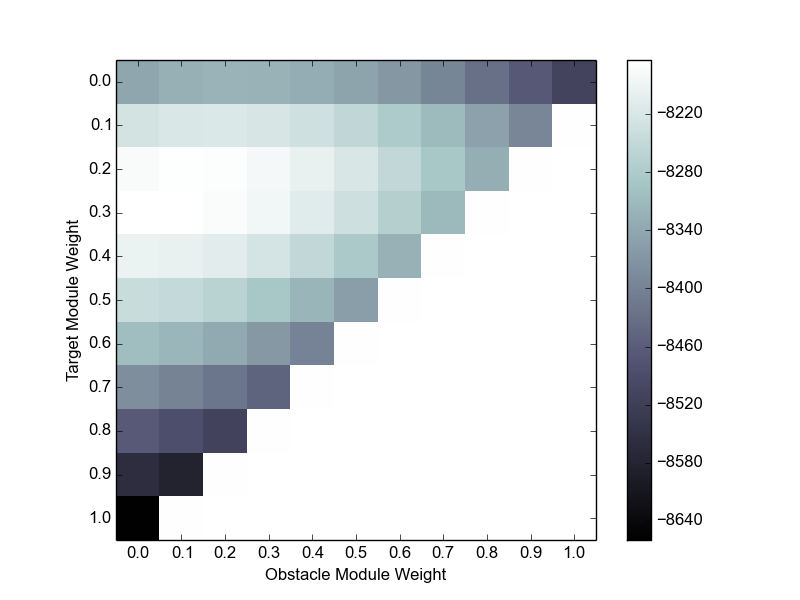
\includegraphics[width=0.4\textwidth]{objValuesTask3.png}
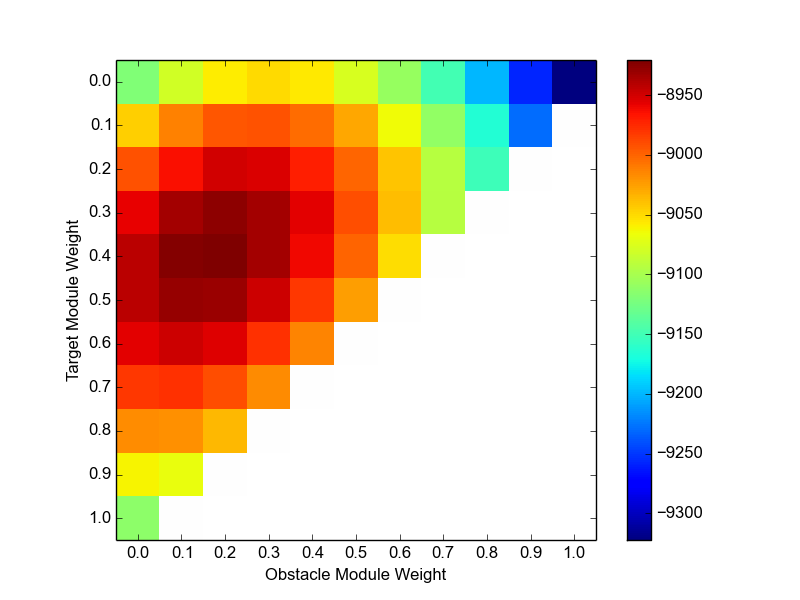
\includegraphics[width=0.4\textwidth]{objValuesTask4.png}
\caption{Heatmaps of the $\log$ of values of Equation~\ref{eq:irl} for different
weights for the four tasks, respectively. The red zones indicate higher values.
The upper two are Task 1 and 2. The lower two are Task 3 and 4.
}
\label{fig:heatmap}
\end{figure}

In Figure~\ref{fig:heatmap}, we show the $\log$ of values of Equation~\ref{eq:irl} for
different weights. We can observe the centroids of red zones move for different
tasks. It stays at the origin in Task 1, so none of target and obstacle modules
are active. It moves away from the origin when a module is active.

From the heatmaps, we find the optimums exist for these tasks. The optimal
weights are also consistent with the experiment context.

\section{Conclusion and Future Work}
\label{sec:conclude}

We interpreted human behavior using inverse module reinforcement learning in
this paper. We have some positive results, but the performance of our agent is
still inferior than humans.

There are also some observations potential for the future work. First, 
weighted sum of Q functions is one way to combine multiple sub-MDPs. We also
propose other ways including, for example, scheduling between different modules,
with only one active at one time. This is also called skilled in the literature
\cite{konidaris2009skill}. However, we adopt the weighted sum approach
because this is more reasonable for human behavior. When a human tries to collect
targets while avoiding obstacles, these two modules are expected to be both
active. A scheduling approach may yield frequent oscillation between these two
modules.

Second, we also assumes independency between modules. Correlation between
modules doesn't impair our analysis in this paper. In Figure~\ref{fig:heatmap},
we can tell that the target module and obstacle module tend to be negatively
correlated from the shape of the red zones.

Lastly, weights may be dynamic and different from state to state. However, with
such assumption, we need to learn a mapping from state to weights. In this case,
the curse of dimensionality still exists, and inverse learning would be
difficult.

\bibliographystyle{plain}
\bibliography{paper}

\end{document}
